%!TEX root = twig-gpu.tex

\section{Code generation}
\label{sec:code-gen}

To generate code, Twig relies on an abstract, language-independent model with a small number of basic operations. This simplified model is useful for formulating Twig's semantics, described in Section~\ref{semantics}. It is also helpful in clarifying the precise operations which Twig supports, without getting bogged down in the (typically quite complicated) details of outputting code for a particular programming language.

Twig generates code in units called \emph{blocks}. The term ``block'' is somewhat overloaded -- our usage differs somewhat from the norm. In Twig, a block of code represents anything that performs some operation on a set of inputs, and which produces a set of outputs. Blocks may have zero or more inputs and outputs. Blocks can also be combined in two different ways: \emph{sequentially}, or \emph{in parallel}. These operations are described in more detail below.

Our current implementation of this model supports the generation of C code, and adds some extra features to support that language. These features include such details as managing type declarations, support for parameterized blocks, and for ``closing'' blocks, which are generated as variables go out of scope and are intended to be used to free resources. We are looking into the possibility of incorporating these and other features into the language-neutral model, but for the moment they are specific to C.

\begin{figure}[ht]
\centering
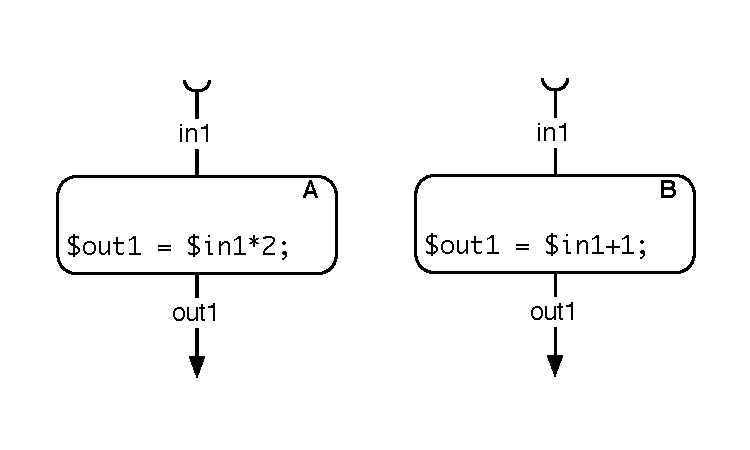
\includegraphics[width=2.5in]{images/code-gen-basic}
\caption{Two basic blocks, $A$ and $B$.}
\label{fig:codegen-blocks}
\end{figure}

\subsection{Block Composition}

As mentioned above, Twig provides two fundamental binary operations on blocks. The first is the \emph{sequential composition} operator, represented by the addition symbol ($+$). Sequencing connects two blocks of code by ``wiring'' the outputs of the first block into the inputs of the second. In C, this is done by creating temporary variables which are substituted into the original blocks. For example, see Figure~\ref{fig:codegen-seq}, which builds on Figure~\ref{fig:codegen-blocks}.

\begin{figure}[ht]
\centering
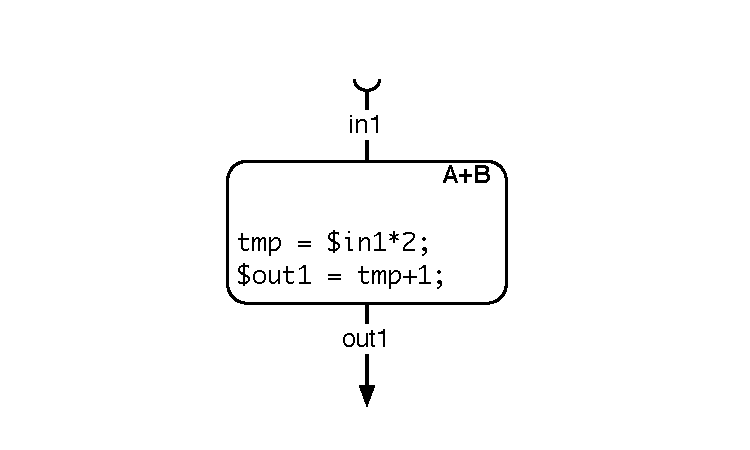
\includegraphics[width=2in]{images/code-gen-seq}
\caption{$A+B$, the sequential composition of blocks $A$ and $B$ from Figure~\ref{fig:codegen-blocks}. A temporary variable is used so that the generated code has the output of $A$ wired to the input of $B$.}
\label{fig:codegen-seq}
\end{figure}

Twig's implementation takes care of declaring and uniquely naming temporary variables to accomplish sequencing.

The second operator is \emph{parallel composition}. Under this operator, two blocks are combined so as to execute independently of one another, but to appear as one single block. We represent this operation with the multiplication operator ($\times$). An example is shown in Figure~\ref{fig:codegen-par}.

\begin{figure}[ht]
\centering
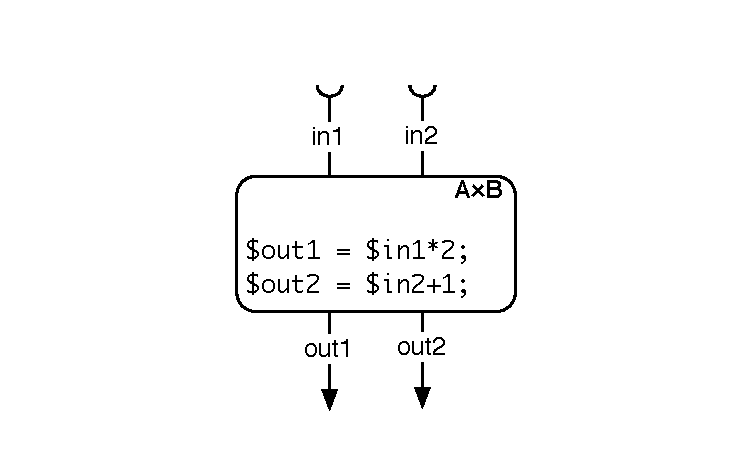
\includegraphics[width=2in]{images/code-gen-par}
\caption{$A \times B$, the parallel composition of blocks $A$ and $B$ from Figure~\ref{fig:codegen-blocks}. Renaming is performed so that the code generated from the composed block has two inputs and two outputs.}
\label{fig:codegen-par}
\end{figure}

\subsection{Identity Blocks}

Twig's formal semantics require the definintion of a set of special \emph{identity} blocks. For each $n \geq 1$, we define an identity block $I_n$ with $n$ inputs and $n$ outputs. Its function is, as its name implies, to simply pass each of its inputs through, unchanged, to the corresponding output. In Twig's semantics we use $I_n$ as a kind of ``no-op.'' We also use $I$ in place of $I_n$ when the value of $n$ is implied from the context.

Identity blocks are subject to a few rules, which we describe here informally and only briefly. First, $I_n$ are left- and right-identity elements under sequential composition, i.e., $I + x = x + I = x$ for all blocks $x$. Second, we can define parallel composition of identity blocks is defined by summing their size, i.e., $I_n \times I_m = I_{n + m}$.

Identity blocks are a special case of \emph{permutation} blocks, which are used to define some combinators in Twig which are not described in this paper. Since we do not need them here, we have elided further details.
